\documentclass[hidelinks,11pt,dvipsnames]{article}
% xcolor commonly causes option clashes, this fixes that
\PassOptionsToPackage{dvipsnames,table}{xcolor}
\usepackage[tmargin=1in, bmargin=1in, lmargin=0.8in, rmargin=1in]{geometry}

%%%%%%%%%%%%%%%%%%%%%%%%%%%%%%%%%%%%%%%%%%%%%%%%%%%%%%%%%%%%%%%%%%%%
%%% For inkscape-figures
%%% Assumes the following directory structure:
%%% master.tex
%%% figures/
%%%     figure1.pdf_tex
%%%     figure1.svg
%%%     figure1.pdf
%%%%%%%%%%%%%%%%%%%%%%%%%%%%%%%%%%%%%%%%%%%%%%%%%%%%%%%%%%%%%%%%%%%%
%\usepackage{import}
\usepackage{pdfpages}
\usepackage{transparent}

\newcommand{\incfig}[2][1]{%
    \def\svgwidth{#1\columnwidth}
    \import{./figures/}{#2.pdf_tex}
}

\pdfsuppresswarningpagegroup=1

% enable synctex for inverse search, whatever synctex is
\synctex=1
\usepackage{float,macrosabound,homework,theorem-env}
\usepackage{microtype}


% font stuff
\usepackage{sectsty}
\allsectionsfont{\sffamily}
\linespread{1.1}

% bibtex stuff
\usepackage[backend=biber,style=alphabetic,sorting=anyt]{biblatex}
\addbibresource{main.bib}

% colored text shortcuts
\newcommand{\blue}[1]{\color{MidnightBlue}{#1}}
\newcommand{\red}[1]{\textcolor{Mahogany}{#1}}
\newcommand{\green}[1]{\textcolor{ForestGreen}{#1}}


% use mathptmx pkg while using default mathcal font
\DeclareMathAlphabet{\mathcal}{OMS}{cmsy}{m}{n}

% fixes the positioning of subscripts in $$ $$
\renewcommand{\det}{\operatorname{det}}

\usetikzlibrary{positioning, arrows.meta}
\newcommand{\here}[2]{\tikz[remember picture]{\node[inner sep=0](#2){#1}}}

%%%%%%%%%%%%%%%%%%%%%%%%%%%%%%%%%%%%%%%%%%%%%%%%%%%%%%%%%%%%%%%%%%%%%
%%% Entry Counter
%%%%%%%%%%%%%%%%%%%%%%%%%%%%%%%%%%%%%%%%%%%%%%%%%%%%%%%%%%%%%%%%%%%%%
\newcounter{entry-counter}
\newcommand{\entry}[1]
{
	\addtocounter{entry-counter}{1}
    \tchap{Entry \arabic{entry-counter}}
	%\addcontentsline{toc}{section}{Entry \arabic{entry-counter}: #1}
	\vspace{-1.5em}
    \begin{center}
		\small \emph{Written: #1}
    \end{center}
}

\usepackage{titling}
\renewcommand\maketitlehooka{\null\mbox{}\vfill}
\renewcommand\maketitlehookd{\vfill\null}


\usepackage{capt-of}
\usepackage{tikz}
\usetikzlibrary{positioning,calc,intersections,through,backgrounds, shapes.geometric, decorations.markings,arrows}

\def\sset{\subseteq}
\def\iso{\cong}
\def\gend#1{\langle #1\rangle}

\newcommand{\rightoverleftarrow}{%
  \mathrel{\vcenter{\mathsurround0pt
    \ialign{##\crcr
      \noalign{\nointerlineskip}$\longrightarrow$\crcr
      \noalign{\nointerlineskip}$\longleftarrow$\crcr
    }%
  }}%
}

\newcommand\makesphere{} % just for safety
\def\makesphere(#1)(#2)[#3][#4]{%
  % Synopsis
  % \makesphere[draw options](center)(initial angle:final angle:radius)
  \shade[ball color = #3, opacity = #4] #1 circle (#2);
  \draw #1 circle (#2);
  \draw ($#1 - (#2, 0)$) arc (180:360:#2 and 3*#2/10);
  \draw[dashed] ($#1 + (#2, 0)$) arc (0:180:#2 and 3*#2/10);
}
% same thing as makesphere but places white background behind
\newcommand\altmakesphere{} % just for safety
\def\altmakesphere(#1)(#2)(#3)[#4][#5]{%
  % Synopsis
  % \make sphere[draw options](center)(initial angle:final angle:radius)
  \draw [fill=white!30] #1 circle (#2);
  \shade[ball color = #4, opacity = #5] #1 circle (#2);
  \draw #1 circle (#2);
  \draw ($#1 - (#2, 0)$) arc (180:360:#2 and 3*#2/10);
  \draw[dashed] ($#1 + (#2, 0)$) arc (0:180:#2 and 3*#2/10);
  \node at #1 {#3};
}

\begin{document}
\pagestyle{empty}
	\LARGE
\begin{center}
	Algebraic Topology Homework 8 \\
	\Large
	Isaac Martin \\
    Last compiled \today
\end{center}
\normalsize
\vspace{-4mm}
\hru

\tchap{Problems from 2.1}

\begin{homework}[e]
  \prob[2.1.4] Compute the simplicial homology groups of the triangular parachute obtained from $\Delta^2$ by identifying its three vertices to a single point.
\begin{prf}
  
  Let $X$ denote the triangular parachute. This space has $1$ vertex, $3$ edges, and $1$ face, so $C_0(X) = \langle v_0\rangle \approx \bZ$, $C_1(X) = \langle a,b,c\rangle \approx \bZ \bigoplus \bZ \bigoplus \bZ$, and $C_2(X) = \langle U \rangle \approx \bZ$. Group homomorphisms are determined by the images of generators, so the chain maps are determined by
  \begin{align*}
    \partial_2(U) &= [v_1,v_2] - [v_0,v_2] + [v_0,v_1] = c - b + a \\
    \partial_1([v_i,v_j]) &= \pm v_i \mp v_j = 0 \\
    \partial_0(v_i) = 0. 
  \end{align*}
  Here, by $\partial_1([v_i,v_j]) = \pm v_i \mp v_j = 0$, we mean that an edge $[v_i,v_j]$ is sent to either $v_i - v_j$ or $-v_i + v_j$, but that this is zero in either case since $v_i = v_j$ in $X$.
  \begin{center}
    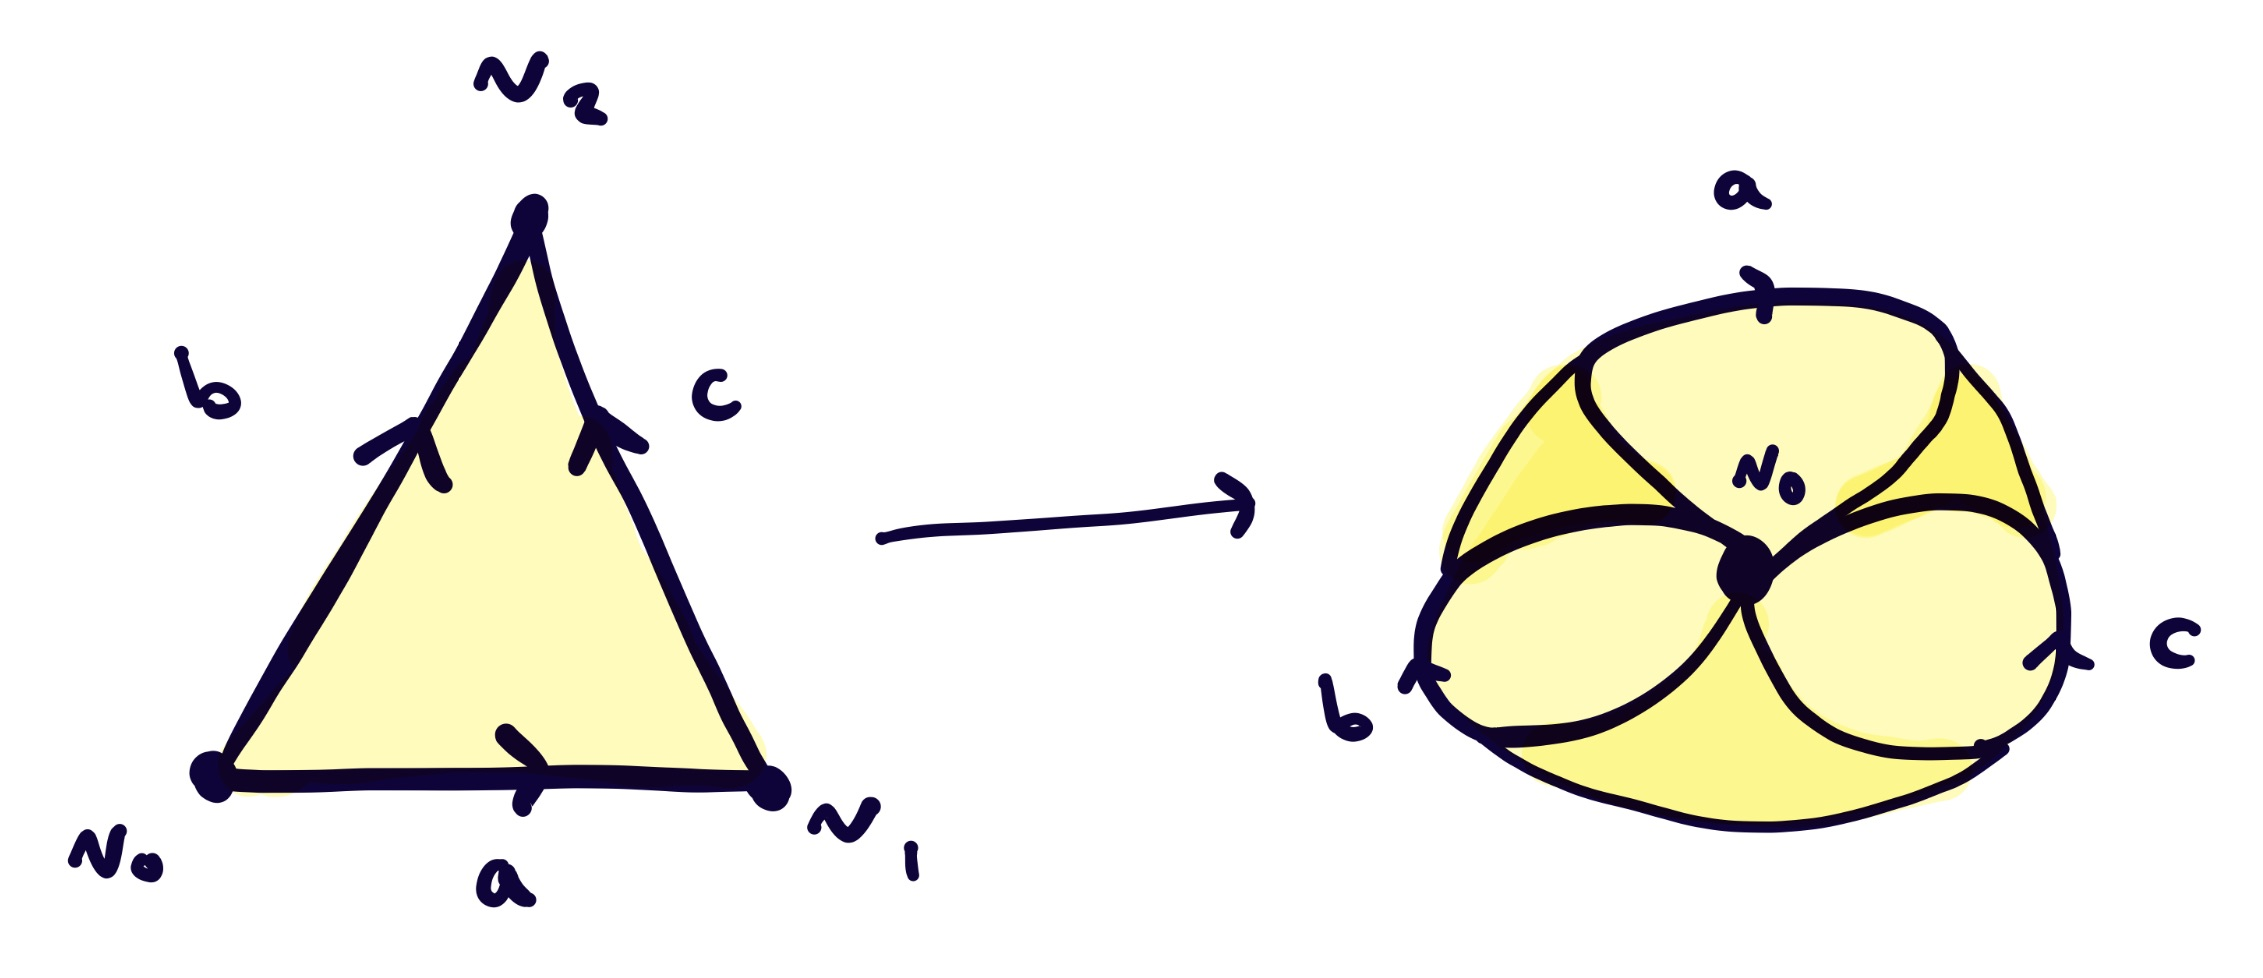
\includegraphics[width=12cm]{figures/hwk8-fig1.png}
    \captionof{figure}{Illustration of the triangular parachute}
    \label{fig:prob1-1}
  \end{center}
  The element $\partial_2(U) = c - b + a$ generates a free group inside $C_1(X)$, hence $\ker(\partial_2) = \{0\}$. As there are no $n$-cells for $n\geq 3$, $\img(\partial_3) = 0$. This means $H_2(X) = \ker(\partial_2) = 0$, the trivial group.

  Since every $1$-cell is mapped to the trivial cycle in $C_0(X)$, $\ker(\partial_1) = C_1(X)$. I claim that $H_1(X) = \ker\partial_1/\img \partial_2 \cong \bZ\oplus \bZ$. To see this, consider the injection $C_2(X) \hookrightarrow C_1(X)$ given by $\partial_2(U) =  c - b + a$. I claim this splits. Indeed, the map $r:C_1(X) \to C_2(X)$ defined $r(a) = U$, $r(b) = -U$, and $r(c) = U$ satisfies $r\circ \partial_2 = \id_{C_2(X)}$ since $r\circ \partial_2(U) = r(a - b + c) = U$. Hence the exact sequence
  \begin{align*}
    0 \to C_2(X) \xrightarrow{\partial_2} C_1(X) \xrightarrow{\pi} C_1(X)/\img \partial_2 \to 0
  \end{align*}
  splits, and $C_2(X) \oplus C_1(X)/\img \partial_2 \cong C_1(X) \cong \bZ^{\oplus 3}$. Because $\bZ^{\oplus 3}$ is torsion free, so also is $C_2(X) \oplus C_1(X)/\img\partial_2$, and in particular so is $C_1(X)/\img \partial_2$. Since $C_2(X) \cong \bZ$ and $C_1(X) \cong \bZ^{\oplus 3}$, by the structure theorem of abelian groups, it must be the case that $C_1(X)/\img\partial_2$ is a rank 2 abelian group, or in other words, is $\bZ^{\oplus 2}$. We therefore have that $H_1(X) = \ker \partial_1/\img\partial_2 = C_1(X)/\img \partial_2 \cong \bZ^{\oplus 2}$.

  Finally, because $X$ is connected, $H_0(X) \cong \bZ$. We conclude that
  \begin{align*}
    H_2(X) \cong \bZ, ~ H_1(X) \cong \bZ\oplus \bZ, ~ H_0(X) \cong \bZ.
  \end{align*}
\end{prf}

\prob[2.1.6] Compute the simplicial horology groups of the $\Delta$-complex obtained from $n+1$ 2-simplicies $\Delta^2_0,...,\Delta^2_n$ by identifying all three edges of $\Delta_0^2$ to a single edge, and for $i > 0$ identifying the edges $[v_0,v_1]$ and $[v_1,v_2]$ of $\Delta_i^2$ to a single edge and the edge of $[v_0,v_2]$ to the edge $[v_0,v_1]$ of $\Delta_{i-1}^2$.
  \begin{prf}
    First we must describe the equivalence classes of the $k$-simplicies. Set $\Delta^2_i = [v_0^i,v_1^i,v_2^i]$.
    \begin{itemize}
      \item \emph{The 0-faces}: ~ For the 0th 2-simplex we have $[v^0_0,v_1^0] \sim [v_1^0,v_2^0]\sim [v_1^0,v^0_2]$ which means that $v^0_0 \sim v^0_1 \sim v^0_2$, and so we may just denote by $v^0$ the equivalence class containing all these vertices.
      \begin{center}
        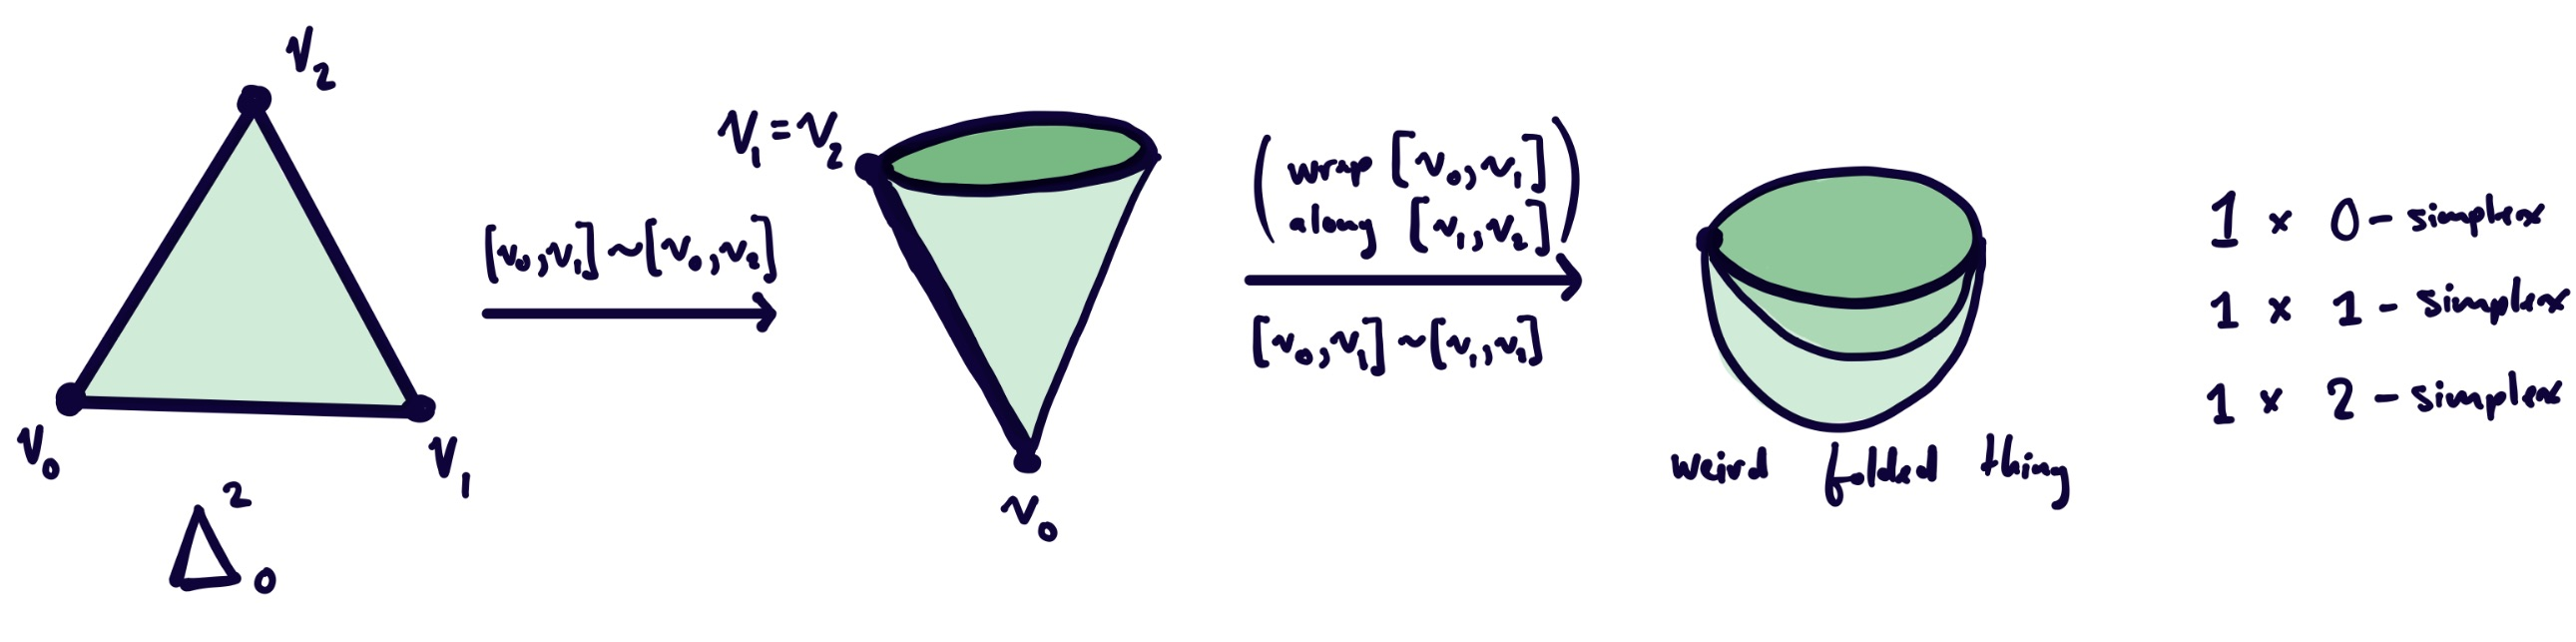
\includegraphics[width=15cm]{figures/hwk8-fig2.png}
        \captionof{figure}{Attempted illustration of the 0th 2-simplex $\Delta^2_0$. The only $1$-simplex is the top-most circle.}
        \label{fig:prob2-1}
      \end{center}
      For the $\Delta^2_1$ simplex, we get that
      \begin{align*}
        [v_0^1,v_2^1] \sim [v_0^0, v_1^0] \implies v^1_0 \sim v_2^1 \sim v^0, \\
        [v_0^1,v_1^1] \sim [v_1^1,v_2^1] \implies v^1_1\sim v^0,
      \end{align*}
      meaning that after performing the identifications for $\Delta_1^2$, we still only have one equivalence class of vertices. Iterating this process, we get that there is only one equivalence class of vertices, $v^0$.

      \item \emph{The 1-faces}: ~ We have one equivalence class containing the three edges from $\Delta^2_0$, denote it by $e_0$. For $\Delta^2_1$, $[v_0^1,v_2^1]$ is identified with $[v_0^0,v_1^0]$ and is therefore in the equivalence class $e_0$, whereas the other two edges are identified with each other to form a new equivalence class $e_1$. For the $\Delta^2_i$ simplex, one edge is ``added'' to $e_i-1$ while its other two edges are identified to form a new equivalence class $e_i$. This gives us $n+1$ equivalence classes of edges, $e_0,e_1,...,e_n$.

      \item \emph{The 2-faces:} ~ No identifications are performed on the $2$-faces, only on their edges. Hence we have $n+1$ equivalence classes of $2$-simplicies, denoted by $U_0,U_1,...,U_n$.
    \end{itemize}
    Now we examine the chain complexes and the boundary maps between them.
    \begin{itemize}
      \item $\partial:C_2\to C_1:$~ We have that
        \begin{align*}
          C_2 = \bZ U_0\oplus ... \oplus \bZ U_n\textbuff{1.5em}{and} C_1 = \bZ e_0\oplus ...\oplus \bZ e_n
        \end{align*}
        with
        \begin{align*}
          \partial(U_0) &= [v^0_1,v^0_2] - [v^0_0,v^0_2] + [v^0_0,v^0_1] = e_0 \\ 
          \partial(U_i) &= [v^i_1,v^i_2] - [v^i_0,v^i_2] + [v^i_0,v^i_1] = 2e_i - e_{i-1}.
        \end{align*}
      \item $\partial:C_1\to C_0:$~ We have $C_0 = \bZ v^0$, so that $\partial(e_i) = v^0 - v^0 = 0$ for all $0\leq i\leq n$. This means $\ker\partial_1 = C_1$.
    \end{itemize}
    All that is left is to compute homology. Since our space is connected, $H_0 = \bZ$, and we already know that $Z_1 = \ker \partial_1 = C_1 = \bZ^{\oplus (n+1)}$, hence all that is left is to find $\ker \partial_2$ and $\img \partial_2$.
    \begin{itemize}
      \item $\ker \partial_2$ and $H_2:$ ~ As noted above, $\partial(U_0) = e_0$ and $\partial(U_i) = 2ei - e_{i-1}$. Hence,
      \begin{align*}
        \partial_2\left(\sum_{i = 0}^n a_iU_i\right) =
        \begin{pmatrix}	
          1 & 0 & 0 & ... & 0 \\ 
          -1 & 2 & 0 & ... & 0 \\
          0 & -1 & 2 & ... & 0 \\
          \vdots & & \ddots & \ddots & \vdots & \\
          0 & 0 & ... & -1 & 2
        \end{pmatrix}\begin{pmatrix} a_0 \\ a_1 \\ \vdots \\ a_n \end{pmatrix}.
      \end{align*}
      This matrix has nonzero determinant, and hence has trivial kernel. Thus, $H_2 = \ker \partial_2 = 0$.
    \item $\img \partial_2$ and $H_1:$ Examining the Smith normal form of the above matrix will prove enlightening. I claim that it is 
      \begin{align*}
        \begin{pmatrix}	
          1 & 0 & ... & 0 & 0 \\
          0 & 1 & ... & 0 & 0 \\
          \vdots & & \ddots & & \vdots \\
          0 & 0 & ... & 1 & 0 \\
          0 & 0 & ... & 0 & 2^n
        \end{pmatrix}.
      \end{align*}
      Assuming the first $i-1$ rows have been diagonalized for $2\leq i$, one can diagonalize the $i$th row via the following row and column operations:
      \begin{align*}
        1&. ~ r_{i-1} = r_{i-1} + (2^n - 1)r_i \\
        2&. ~ r_i = r_i + r_{i-1} \\
        3&. ~ c_i = c_i - (2^n - 1)\cdot 2 c_{i-1}.
      \end{align*}
      To see this, we need only consider a $2\times 2$ matrix whose diagonal elements line up with the matrix defining $\partial_2$. Set $k = i - 2$ to simplify notation:
      \begin{align*}
        \begin{pmatrix}	
          2^k & 0 \\
          -1 & 2
        \end{pmatrix}\sim
        \begin{pmatrix}
          1 & (2^k - 1)\cdot 2 \\
          -1 & 2
        \end{pmatrix}\sim
        \begin{pmatrix}
          1 & (2^k - 1)\cdot 2 \\
          0 & 2^k
        \end{pmatrix}
        \begin{pmatrix}
          1 & 0 \\
          0 & 2^{k+1}
        \end{pmatrix}.
      \end{align*}
      From the Smith normal form of $\partial_2$, it is easy to see that $\partial_2$ has image isomorphic to $\bZ e_0 \oplus ... \oplus \bZ e_{n-1} \oplus 2^n\bZ e_{n}$ in $C_1$. Hence,
      \begin{align*}
        H_1 \cong \bZ/2^{n}\bZ.
      \end{align*}
  \end{itemize}
  We conclude that $H_0 \cong \bZ$, $H_1 \cong \bZ/2^{n}\bZ$ and $H_2 \cong 0$.
  \end{prf}
  \prob[2.1.7] Find a way of identifying pairs of faces of $\Delta^3$ to produce a $\Delta$-complex structure on $S^3$ having a single $3$-simplex, and compute the simplicial homology groups of this $\Delta$-complex.
  \begin{prf}
    Let $\Delta^3 = [0 1 2 3]$ be the $3$-simplex in question. It's boundary is the 2-chain $[123] - [023] + [013] - [012]$. Intuitively, $S^3$ ought to have homology $H_0 = H_3 = \bZ$ with trivial homology everywhere else, since it is connected and encompasses only a 3-dimensional hole, so the vibe-motivated identification to make is $[123] = [023]$ and $[013] = [012]$.
    \begin{center}
      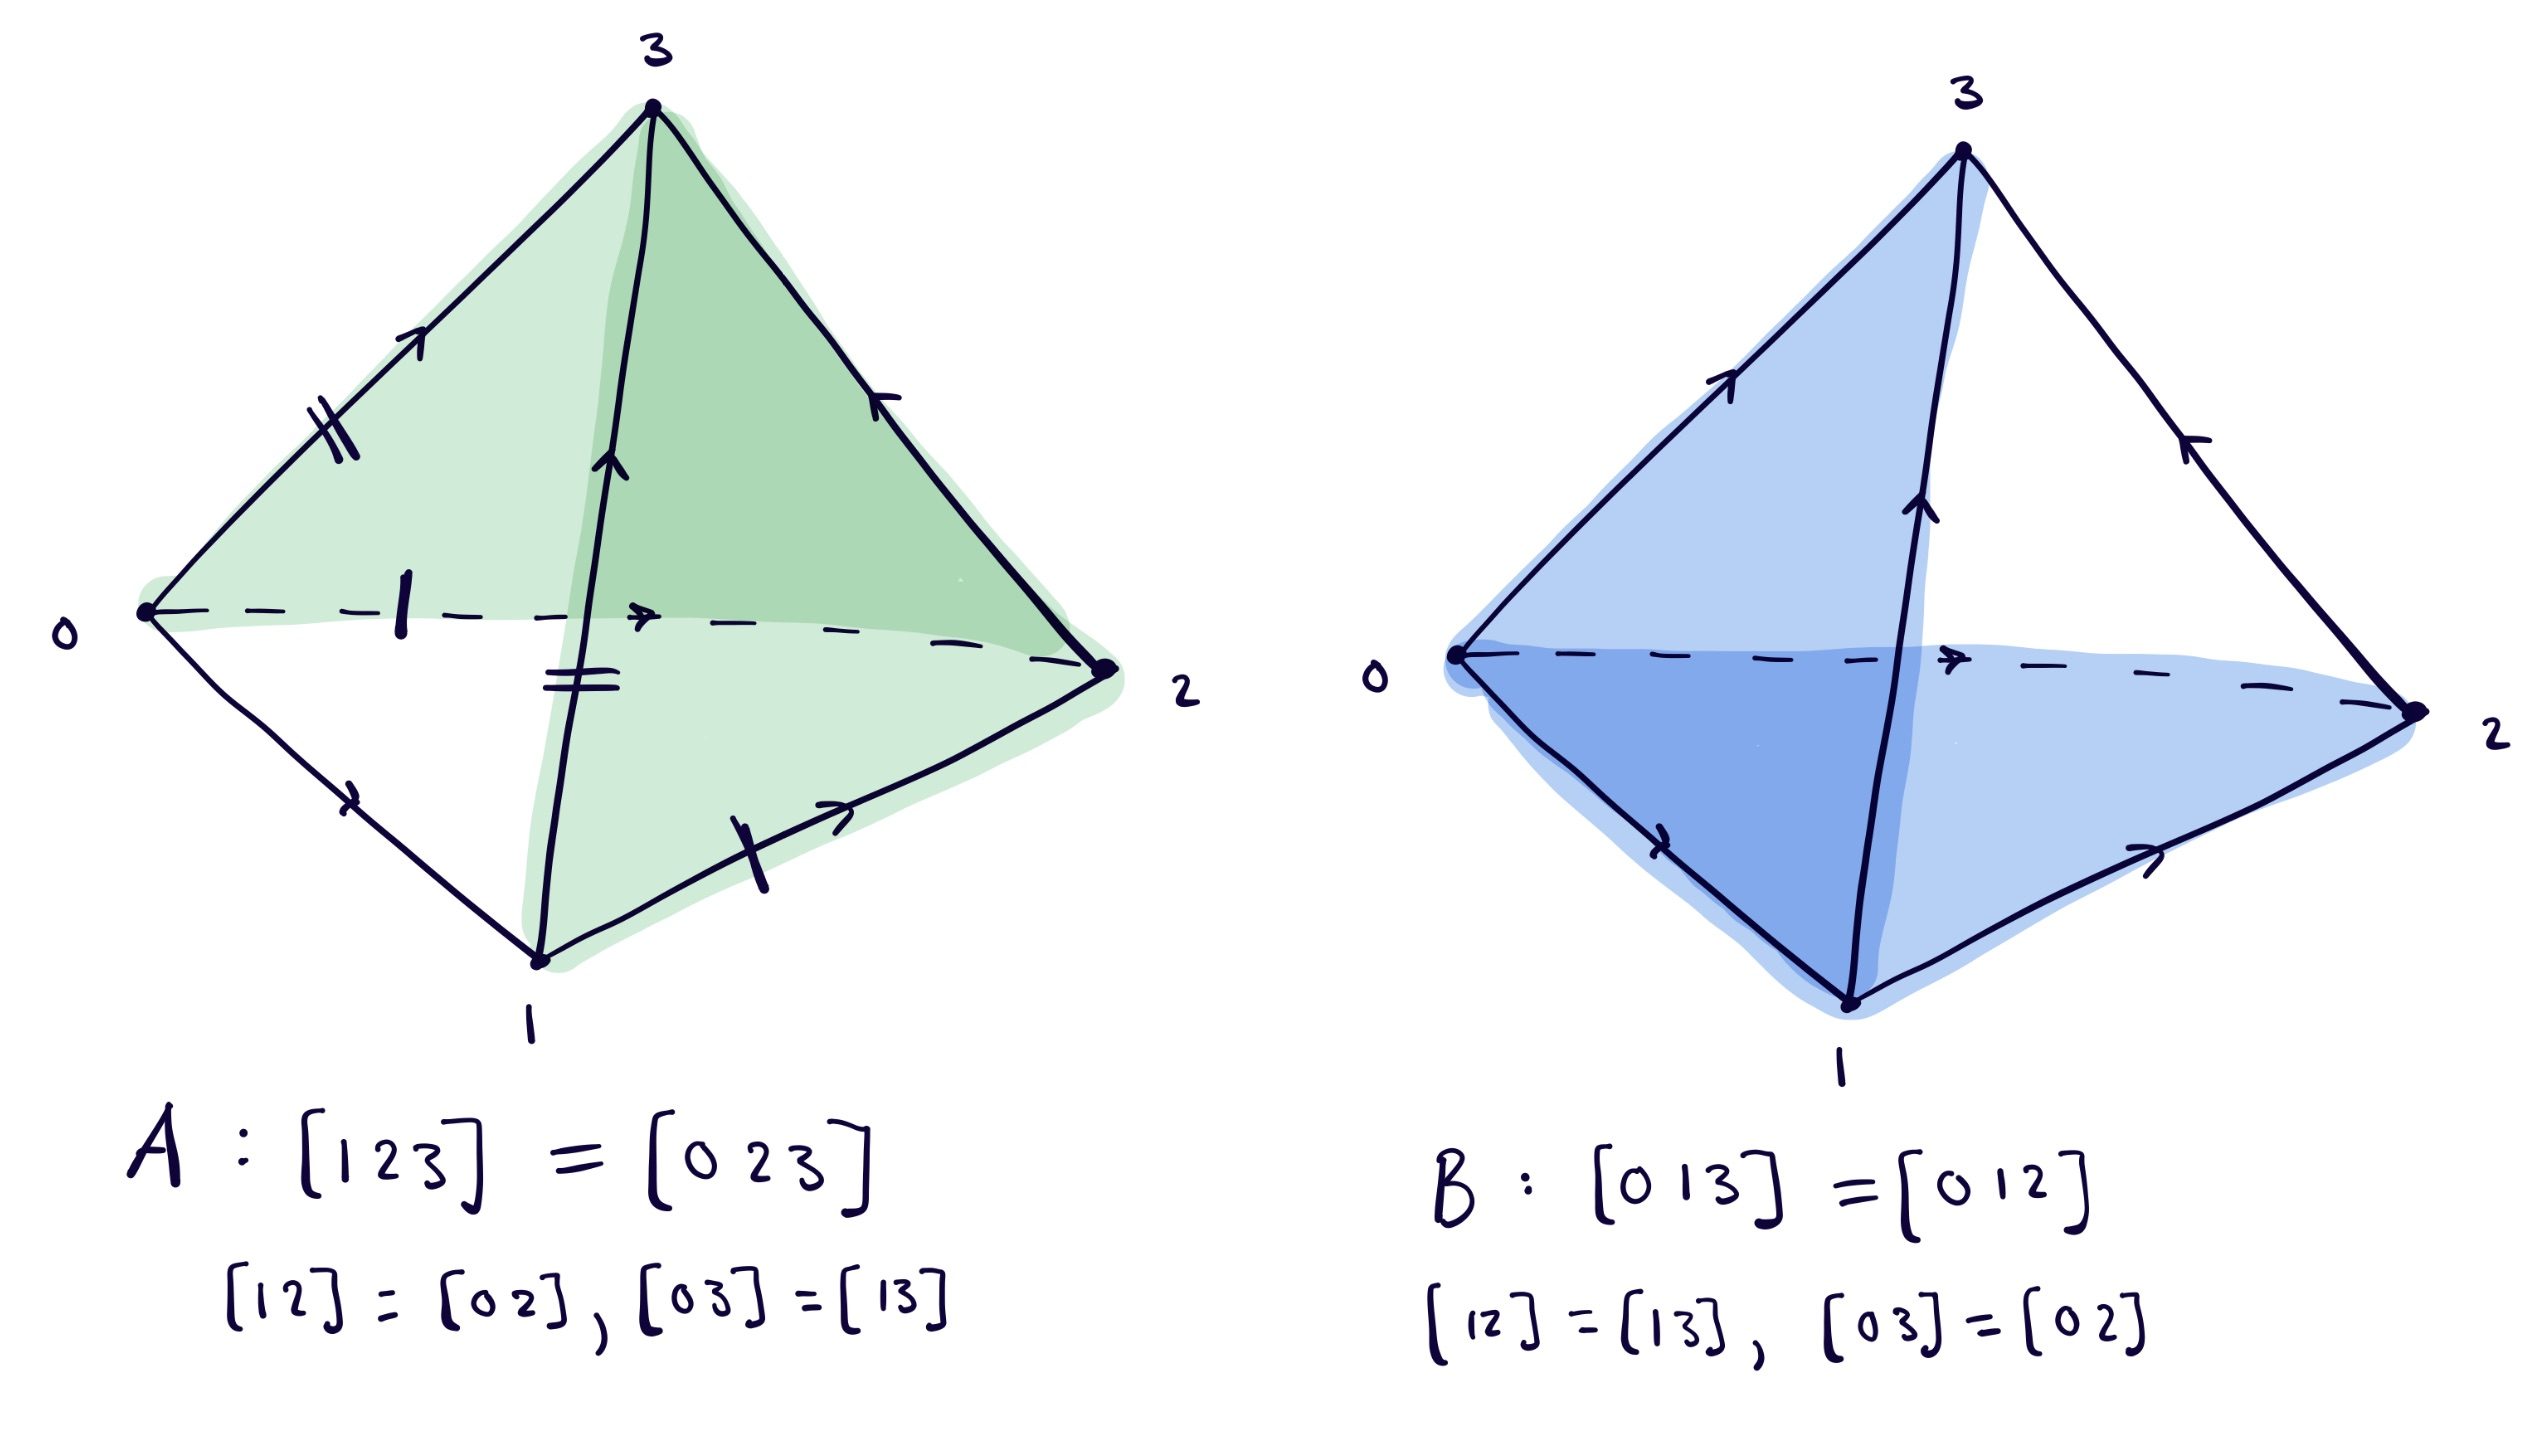
\includegraphics[width=15cm]{figures/hwk8-fig4.png}
      \captionof{figure}{The identification discussed above.}
      \label{fig:prob3-1}
    \end{center}

    I claim that this is the (or a?) correct identification to make. Call the resulting space $X$, and note that it has 1 $\times$ 3-simplex, $2$ $\times$ 2-simplicies,
    \begin{align*}
      A&: ~[123] = [023] \\
      B&: ~[013] = [012],
    \end{align*}
    3 $\times$ 1-simplicies,
    \begin{align*}
      a:[01], ~ b: [13] = [03] = [12] = [02], ~ c:[23]
    \end{align*}
    and 2 $\times$ 0-simplicies, $x: 0 = 1$ and $y: 2 = 3$. We can write out the simplicial chain complex quite explicitly now:
    \begin{align*}
      0 \to \bZ \xrightarrow{0} \bZ\{A,B\} \xrightarrow{
        \begin{pmatrix}	1 & 0 \\ 0 & 0 \\ 0 & 1  \end{pmatrix}
      } \bZ\{a,b,c\} \xrightarrow{
        \begin{pmatrix}	0 & 1 & 0 \\ 0 & -1 & 0 \end{pmatrix}
      } \bZ\{x,y\} \to 0.
    \end{align*}
    To see that this does in fact produce a space homeomorphic to $S^3$, let's examine the identifications a little more closely. After rotating $X$, we see that we have two cones identified at their faces:
    \begin{center}
      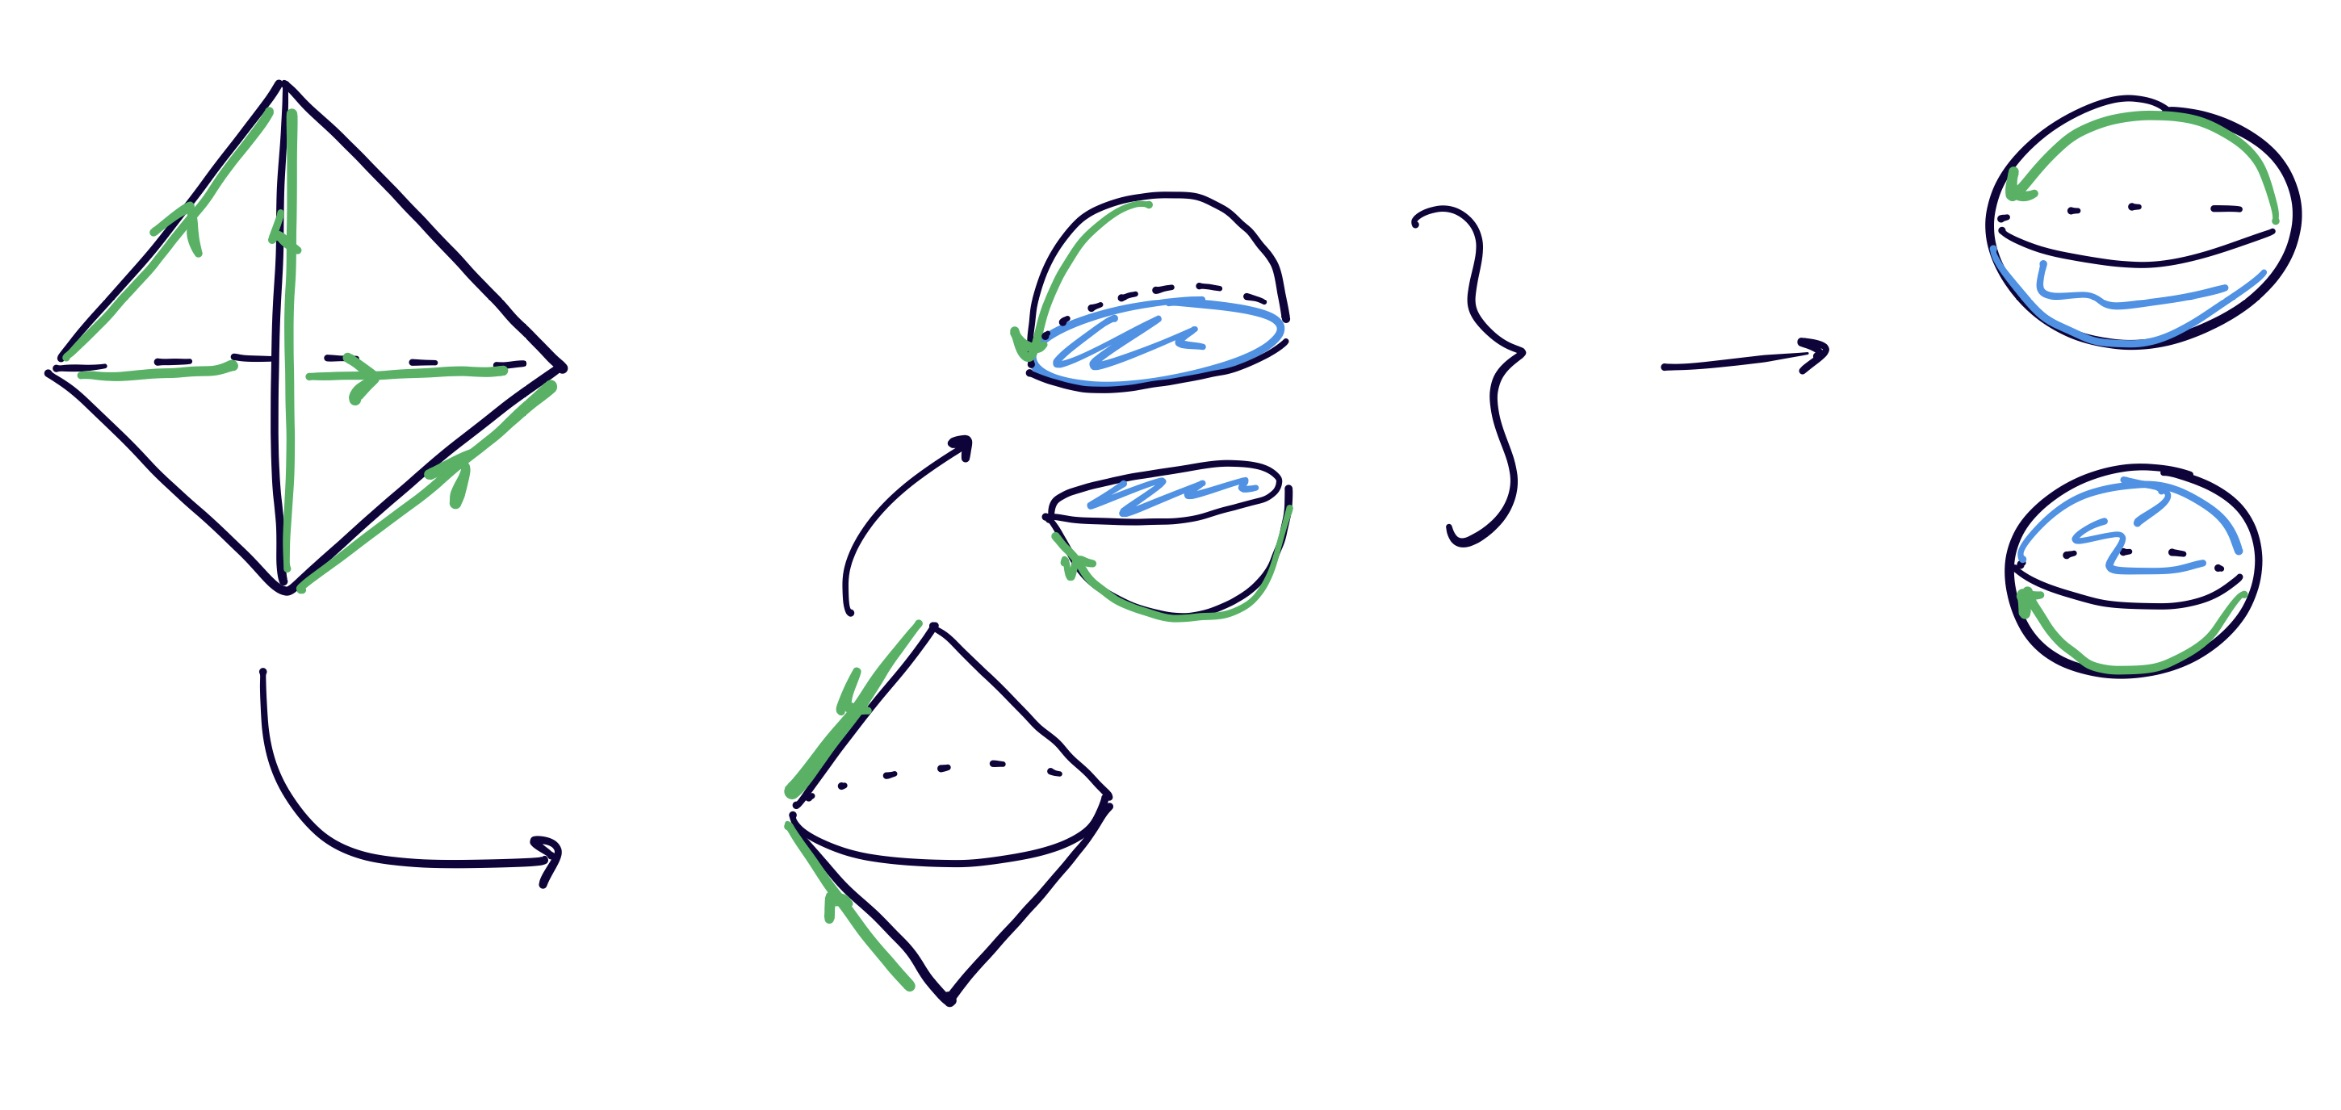
\includegraphics[width=15cm]{figures/hwk8-fig5.png}
      \captionof{figure}{The space $X$ is homeomorphic to two 3-disks identified along their boundary}
      \label{fig:prob3-2}
    \end{center}
    which gives us two disks identified along their boundary, i.e. $S^3$. Since $\partial_3$ is the zero map by definition, $H_3(X) \cong \bZ\{[0123]\} \cong \bZ$. The map $\partial_2$ is given by multiplication over a rank 2 matrix, and hence has trivial kernel implying $H_2(X) = 0$. The kernel of $\partial_1$ is generated by $a$ and $c$, but these are the images of $A$ and $B$ respectively over $\partial_2$, hence $\ker\partial_1 = \img \partial_2\implies H_1(X) = 0$. Finally, $H_0(X)$ is $\bZ$ since $X$ is path-connected.

  \end{prf}
  \prob[2.1.8] Construct a 3-dimensional $\Delta$-complex $X$ from $n$ tetrahedra $T_1,...,T_n$ by the following two steps. First arrange the tetrahedra in a cyclic pattern as in the figure, so that each $T_i$ shares a common vertical face with its two neighbors $T_{i-1}$ and $T_{i+1}$ subscripts being taken mod $n$. Then identify the bottom face of $T_i$ with the top face of $T_{i+1}$ for each $i$. Show the simplicial homology groups of $X$ in dimensions $0,1,2$ and $3$ are $\bZ,\bZ_n, 0$ and $\bZ$ respectively.
  \begin{prf}
    I tried to draw this space, but honestly found the drawing more confusing than enlightening. The solution to this problem essentially boils down to carefully understanding the boundary maps and the identifications between simplicies, which can be done entirely symbolically. I included a screencap of the diagram in Hatcher for reference.
    \begin{center}
      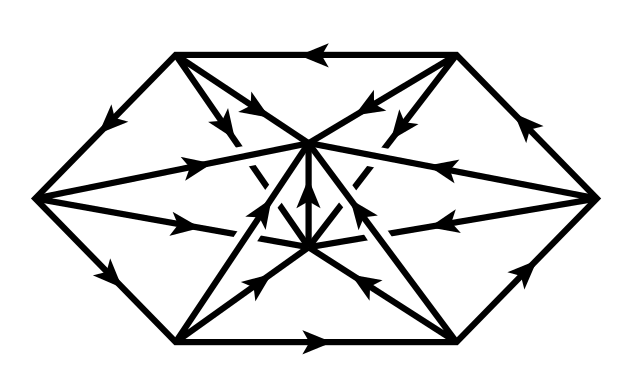
\includegraphics[width=10cm]{figures/hwk8-fig3.png}
      \captionof{figure}{Tetrahedra arranged in a cyclic pattern (page 131 Hatcher)}
      \label{fig:prob4-1}
    \end{center}
    By constructing $X$ above from $n$ $3$-simplicies as suggested, we end up with
    \begin{itemize}
      \item $n$ $\times$ 3-simplicies, $T_1,...,T_n$
      \item $2n$ $\times$ $2$-simplicies, $E_1,...,E_n$ (exterior 2-simplicies) and $I_1,...,I_n$ (interior $2$-simplicies)
      \item $(n+2)$ $\times$ $1$-simplicies $d_1$,...,$d_n$ oriented diagonally, $h$ oriented horizontally and $v$ oriented vertically. This vertically oriented edge corresponds to the edge in the interior of the diagram from Hatcher.
      \item $2$ $\times$ $0$-simplicies, call them $x$ and $y$.
    \end{itemize}
    Following the identifications, we see that the boundary maps are
    \begin{align*}
      \partial_3(T_i) = I_i - I_{i-1} + E_i - E_{i+1} \\
    \end{align*}
    \begin{align*}
      \partial_2(I_i) = v - d_i  + d_{i+1}, \hspace{1em} \partial_2(E_i) = d_i - d_{i-1} + h \\
    \end{align*}
    \begin{align*}
      \partial_1(d_i) = y - x, \hspace{1em} \partial_1(h) = 0, \hspace{1em} \partial_1(v) = 0.
    \end{align*}
    Note that if $i = 1$ then $i - 1$ is meant to mean $i = n$ and if $i = n$ then $i + 1$ is meant to mean $1$, that is, consider the indices mod $n$.

    Let us first examine the kernel of $\partial_3$. We can rewrite the image of an arbitrary $3$-chain $\sum_{i=1}^n a_i T_i$ under $\partial_3$ as follows:
    \begin{align*}
      \partial_3\left(\sum_{i=1}^n a_i T_i\right) 
      &= \sum_{i=1}^n a_i(I_i - I_{i-1} + E_i - E_{i+1}) \\
      &= \sum_{i=1}^n (a_i - a_{i+1})I_i ~+~ \sum_{i=1}^n (a_i - a_{i-1})E_i.
    \end{align*}
    If $\partial_3\left(\sum_{i=1}^n a_i T_i\right) = 0$, it must therefore be the case that $a_{i-1} = a_i = a_{i+1}$, so that $\sum_{i=1}^n a_i T_i = a(T_1+ ... + T_n)$ for some integer $a \in \bZ$. It follows that $\ker \partial_3 = \bZ(T_1+...+T_n)$, and hence $H_3(X) = \ker\partial_3 \cong \bZ$.

    Let's now determine $\ker \partial_2$ and $H_2(X)$. As before, let's consider the image of an arbitrary $2$-chain $c = \sum_{i=1}^n a_iI_i ~+~ \sum_{i=1}^n b_iE_i$ under $\partial_2$:
    \begin{align*}
      \partial_2\left(\sum_{i=1}^n a_iI_i ~+~ \sum_{i=1}^n b_iE_i\right) 
      &= \sum_{i=1}^n a_i(v - d_i + d_{i+1}) + b_i(d_i - d_{i-1} + h) \\
      &= \sum_{i=1}^n (b_{i} - b_{i+1} + a_{i-1} - a_i)d_i ~+~ (a_1+b_1+...+a_n+b_n)(v + h).
    \end{align*}
    If $\partial_2(c) = 0$, then we have
    \begin{align*}
      (b_{i}-b_{i+1}+a_{i-1}-a_i) = 0, \textbuff{1em}{and}(a_1 + b_1 + ... + a_n + b_n) = 0.
    \end{align*}
    This first condition implies $b_i + a_{i-1} = b_{i+i} + a_{i}$ for all $i$, so $b_i + a_{i-1}= \alpha$ for some constant $\alpha \in \bZ$. The second condition gives us
    \begin{align*}
      a_1 + b_1 + ... + a_n + b_n = n \alpha = 0
    \end{align*}
    in $\bZ$. But $\bZ$ is an integral domain, so $\alpha = 0 \implies b_i = -a_{i-1}$ for all $1\leq i\leq n$, remembering our convention that indices are valued in $\{1,...,n\}$ and are computed mod $n$. This implies that
    \begin{align*}
      \ker\partial_2 = \bZ\langle E_i - I_{i-1} \mid i\in \{1,...,n\}\rangle.
    \end{align*}
    Each of these is the image of some $3$-chain, and hence $H_2(X) = \ker\partial_2/\img\partial_3 \cong 0$.

    \bigskip

    Our last task is to compute $H_1$. Consider the image of an arbitrary $1$-chain $a_1d_1+...+a_nd_n + bv+ch$:
    \begin{align*}
      \partial_1(a_1d_1+...+a_nd_n + bv+ch) = (a_1+...+a_n)(y - x).
    \end{align*}
    This is equal to $0$ if and only if $a_1+...+a_n = 0$. Notice that $d_i - d_{i-1} \in \ker\partial$, and that if $a_1+ ... + a_n = 0\implies a_n = -a_1 - ... - a_{n-1}$,
    \begin{align*}
      \sum_{i=0}^nb_i (d_i - d_{i-1}) = \sum_{i=1}^n (b_i - b_{i+1})d_i = \sum_{i=1}^n a_i d_i
    \end{align*}
    if we set $b_1 = 0$ and $b_{i+1} = b_i - a_i$. This gives us a much more convenient set of generators for $\ker\partial_2$:
    \begin{align*}
      \ker\partial_2 = \bZ\langle d_2-d_1, d_3-d_2,...,d_n-d_{n-1},h,v \rangle.
    \end{align*}
    From the description of $\partial_2$ at the beginning of the problem, we get that
    \begin{align*}
      \partial_2(E_1 + ... + E_n) = (h + d_1 - d_n) + (h + d_2 - d_1) + ... + (h + d_n - d_{n-1}) = nh.
    \end{align*}
    We also have that $\partial_2(E_2 + I_1) = h - v$, so $h = v$ in $H_1(X) = \ker \partial_1/\img(\partial_2)$. I'm not quite sure how to see that each 1-chain of the form $d_i - d_{i-1}$ is in $\img\partial_2$, but we see that we're only a summand of $h$ or $v$ off from having this directly. Once we have this fact, we get that
    \begin{align*}
      H_1(X) = \ker\partial_1/\img\partial_2 \cong h\bZ/nh\bZ \cong \bZ/n\bZ.
    \end{align*}
    Finally, because $X$ is path connected, $H_0(X) \cong \bZ$.

  \end{prf}
  \prob[2.1.11] Show that if $A$ is a retract of $X$ then the map of $H_n(A)\to H_n(X)$ induced by the inclusion $A\subseteq X$ is injective.
  \begin{prf}
    First recall the two basic functorial properties of induced homomorphisms on homology from page 111 of Hatcher:
    \begin{enumerate}[(i)]
      \item $(fg)_* = f_*g_*$ for compositions $X\xrightarrow{f}Y\xrightarrow{g}Z$ and
      \item $(\id_X)_* = \id_{H_n(X)}$.
    \end{enumerate}
    If $A$ is a retract of $X$, then the inclusion $\iota:A\to X$ has a left inverse $r:X\to A$, in which case the induced map of the composition is
    \begin{align*}
      \id_{H_n(X)} = (\id_X)_* = (r\circ \iota)_* = r_*\circ \iota_*.
    \end{align*}
    The injectivity of $\iota_*$ then follows from the injectivity of $\id_{H_n(X)}$.
  \end{prf}
  \prob[2.1.12] Show that chain homotopy of chain maps is an equivalence relation.
  \begin{prf}
    Two maps $f,g:C_n \to C'_n$ are chain homotopic (via a map $P$) if there exists a map $P:C_n \to C_{n+1}'$ such that $\partial P - P\partial = g - f$, where these maps are defined for all values of $n$. We verify that the relation ``$f \sim g$ if $f$ and $g$ are chain homotopic'' is an equivalence relation of chain maps.
    \begin{itemize}
      \item Reflexivity. ~ Suppose $f$ is a chain map and $P:C_n\to C_{n+1}'$ is the zero map. Then
        \begin{align*}
          \partial P + P \partial = 0 = f - f,
        \end{align*}
        so $f$ is chain homotopic to itself.
      \item Suppose $f \sim g$, so that there is some map $P:C_n \to C_{n+1}'$ such that $\partial P + P \partial = g - f$. Define $Q = -P$. This is still a homomorphism since multiplication by $-1$ is a $\bZ$-module homomorphism and hence a homomorphism of abelian groups. Thus
        \begin{align*}
          \partial Q + Q\partial = \partial (-P) + (-P)\partial = - (g - f) = f - g,
        \end{align*}
        and $g \sim f$.
      \item Transitivity. ~ Let $f,g,h:C_n \to C_n'$ be chain maps with $f \sim g$ via $P$ and $g \sim h$ via $Q$. Consider the homomorphism $P + Q:C_n \to C_{n+1}'$. Since $\partial$ is a homomorphism we have
        \begin{align*}
          \partial(P+Q) (P+Q)\partial = \partial P + P\partial + \partial Q  + Q\partial = g - f + h - g = h - f,
        \end{align*}
        so $f \sim h$ via $P + Q$.
    \end{itemize}

  \end{prf}
  \prob[2.1.13] Verify that $f \simeq g$ implies $f_* = g_*$ for induced homomorphisms of reduced homology groups.
  \begin{prf}
    We have seen that when $f\simeq g$, the induced maps $f_\sharp$ and $g_\sharp$ on chain complexes are chain-homotopic. This means there exist maps $P_n:C_n(X) \to C_{n+1}(Y)$ such that $\partial P_n + P_n \partial = g_\sharp - f_\sharp$ for all $n\geq 0$. Implicitly, $\partial_0 = 0$, so $\partial P_0 = f_\sharp - g_\sharp$. To show $f_* = g_*$ on reduced homology, it suffices to show that $f_\sharp$ and $g_\sharp$ remain chain homotopic on the extended chain complex.

    Therefore, let $f,g:X\to Y$ be homotopic maps and let $P_n:C_n(X) \to C_{n+1}(Y)$ be the chain homotopy between them. We want to find another map $Q$ so that
    \begin{center}
      \begin{tikzcd}
        ... \arrow[r] & C_2(X) \arrow[r,"\partial"] \arrow[ld,"P_2"] & C_1(X) \arrow[r,"\partial"] \arrow[ld,"P_1"]& C_0(X) \arrow[r,"\epsilon"] \arrow[ld,"P_0"] & \bZ \arrow[r] \arrow[ld,"Q"] & 0 \\
        ... \arrow[r] & C_2(Y) \arrow[r,"\partial"] & C_1(Y) \arrow[r,"\partial"] & C_0(Y) \arrow[r,"\epsilon"] & \bZ \arrow[r] & 0 \\
      \end{tikzcd}
    \end{center}
    is a chain homotopy. This is already a chain homotopy everywhere except at the last square, so we need only find $Q$ such that
    \begin{enumerate}[(1)]
      \item $\partial P_0 + Q \epsilon = f_\sharp - g_\sharp$
      \item $\epsilon Q = f_\sharp - g_\sharp = 0$.
    \end{enumerate}
    However, since the complex is exact at $\bZ$, $\epsilon$ is injective and hence condition (2) above forces $Q = 0$. This definition for $Q$ satisfies (1) since we already have $\partial P_0 = f_\sharp - g_\sharp$. Thus, $f_\sharp$ and $g_\sharp$ are chain homotopic on the extended complex and thus $f_* = g_*$ on reduced homology.
  \end{prf} 
\end{homework}
\end{document}
